\documentclass[a4paper, 12pt, titlepage]{article}

% Document quality things
\usepackage[utf8]{inputenc}
\usepackage{microtype}
\usepackage[dvipsnames]{xcolor}
\usepackage{csquotes, verbatim}
\usepackage{url, hyperref}
\hypersetup{colorlinks=true, linkcolor=black, citecolor=black, urlcolor=blue}

% Image-related packages
\usepackage{graphicx}
%\usepackage{float}
\graphicspath{{./gfx/}}
%\usepackage[font=small,skip=5pt]{caption}

% Setting margins
\usepackage[a4paper,bottom=2cm,top=2cm,left=2.5cm,right=2.5cm, includefoot]{geometry}

% Table helper packages
%\usepackage{multirow, multicol}
%\usepackage{makecell}
%\usepackage{array}
%\usepackage{tabularx} % Not needed currently, but has a few nice options
%\usepackage{wrapfig} % Floating figures/tables
%\usepackage{booktabs}
%\usepackage{catchfile}

% Prevents spamming tedious newlines everywhere, also disables auto indentation, etc.
\usepackage[skip=0.75\baselineskip plus 2pt]{parskip}

% Self-explanatory
%\usepackage{titlesec}
%\titleformat{\section}[block]{\normalfont\scshape\Large}{\thesection}{1em}{}
%\titleformat{\subsection}{\normalfont\large}{\thesubsection}{1em}{}

% Plotting package
\usepackage{pgfplots}
\pgfplotsset{compat = newest}

\begin{document}
  \begin{center}
    {\Large CS 319 - Object-Oriented Software Engineering}\\
    {\vspace{1.5em}\large Design Patterns Homework}\\
    {Vedat Eren Arıcan - 22002643}
  \end{center}
  
  \section{Design Patterns Identified}
  
  \subsection{Decorator Pattern}
  
  The options (i.e., \texttt{TrackElapsedTime}) that are available for \textit{decorating} a task instance are fit for the use of this pattern.
  They present a need to be able to add functionality to an existing type.
  Particularly of note is that these options can be \textbf{combined}, which this pattern lets us do.
  
  \textbf{Implementation:} \texttt{BaseTodoTaskDecorator}, \texttt{TimeTrackingDecorator},\\ \texttt{StatusHistoryDecorator}
  
  \subsection{Strategy Pattern}
  
  The various ways in which a list can have its contents sorted is fit for the use of this pattern.
  Note that there should only be one way of sorting for a given list, which is possible with a single strategy.
  
  \textbf{Implementation:} \texttt{ITodoTaskSortingStrategy}, \texttt{BaseTodoTaskSortingStrategy},\\
  \texttt{AlphabeticalSortingStrategy}, \texttt{AddOrderSortingStrategy},\\ \texttt{TargetDateSortingStrategy}
  
  \subsection{Composite Pattern}
  
  Each list can store tasks and other lists within. Since these nested lists may have other objects inside,
  we can see a clear tree-like structure. This calls for the composite pattern.
  
  \textbf{Implementation:} \texttt{ITodoComponent}, \texttt{ITodoTask}, \texttt{TodoList}
  
  \subsection{State Pattern}
  
  The various states a task can take are fit for the use of this pattern.
  We can model the \textit{created}, \textit{in progress}, \textit{completed} states this way.
  
  \textbf{Implementation:} \texttt{ITodoTaskState}, \texttt{CreatedState}, \texttt{InProgressState},\\ \texttt{CompletedState}
  
  \pagebreak
  \section{Class Diagram}
  
  Note that the diagram below is in vector format.
  It can be zoomed into without hurting picture quality.
  \vspace{2em}
  
  \begin{center}
    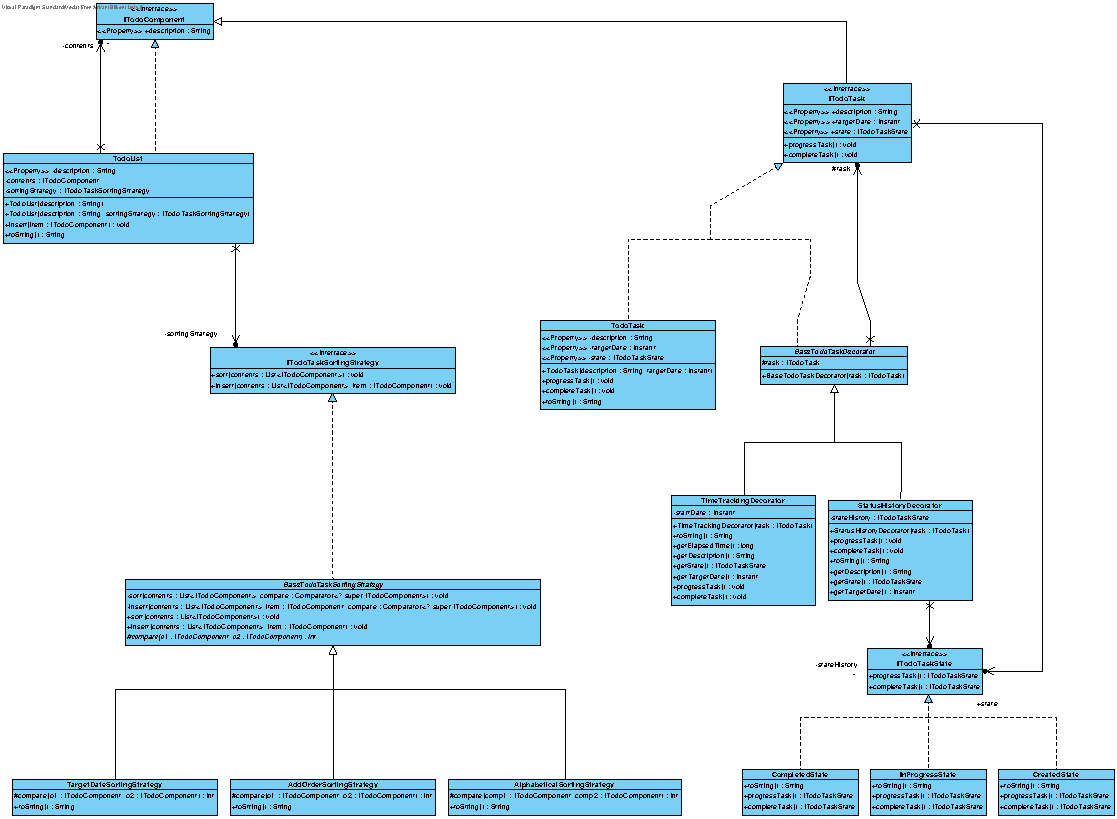
\includegraphics[width=\textwidth]{class_diag}
  \end{center}
  
\end{document}
